\documentclass[11pt]{article}
\pagestyle{empty}
\setlength{\parindent}{0pt}
\usepackage[simplified]{pgf-umlcd}
\usepackage{tikz}

\begin{document}
    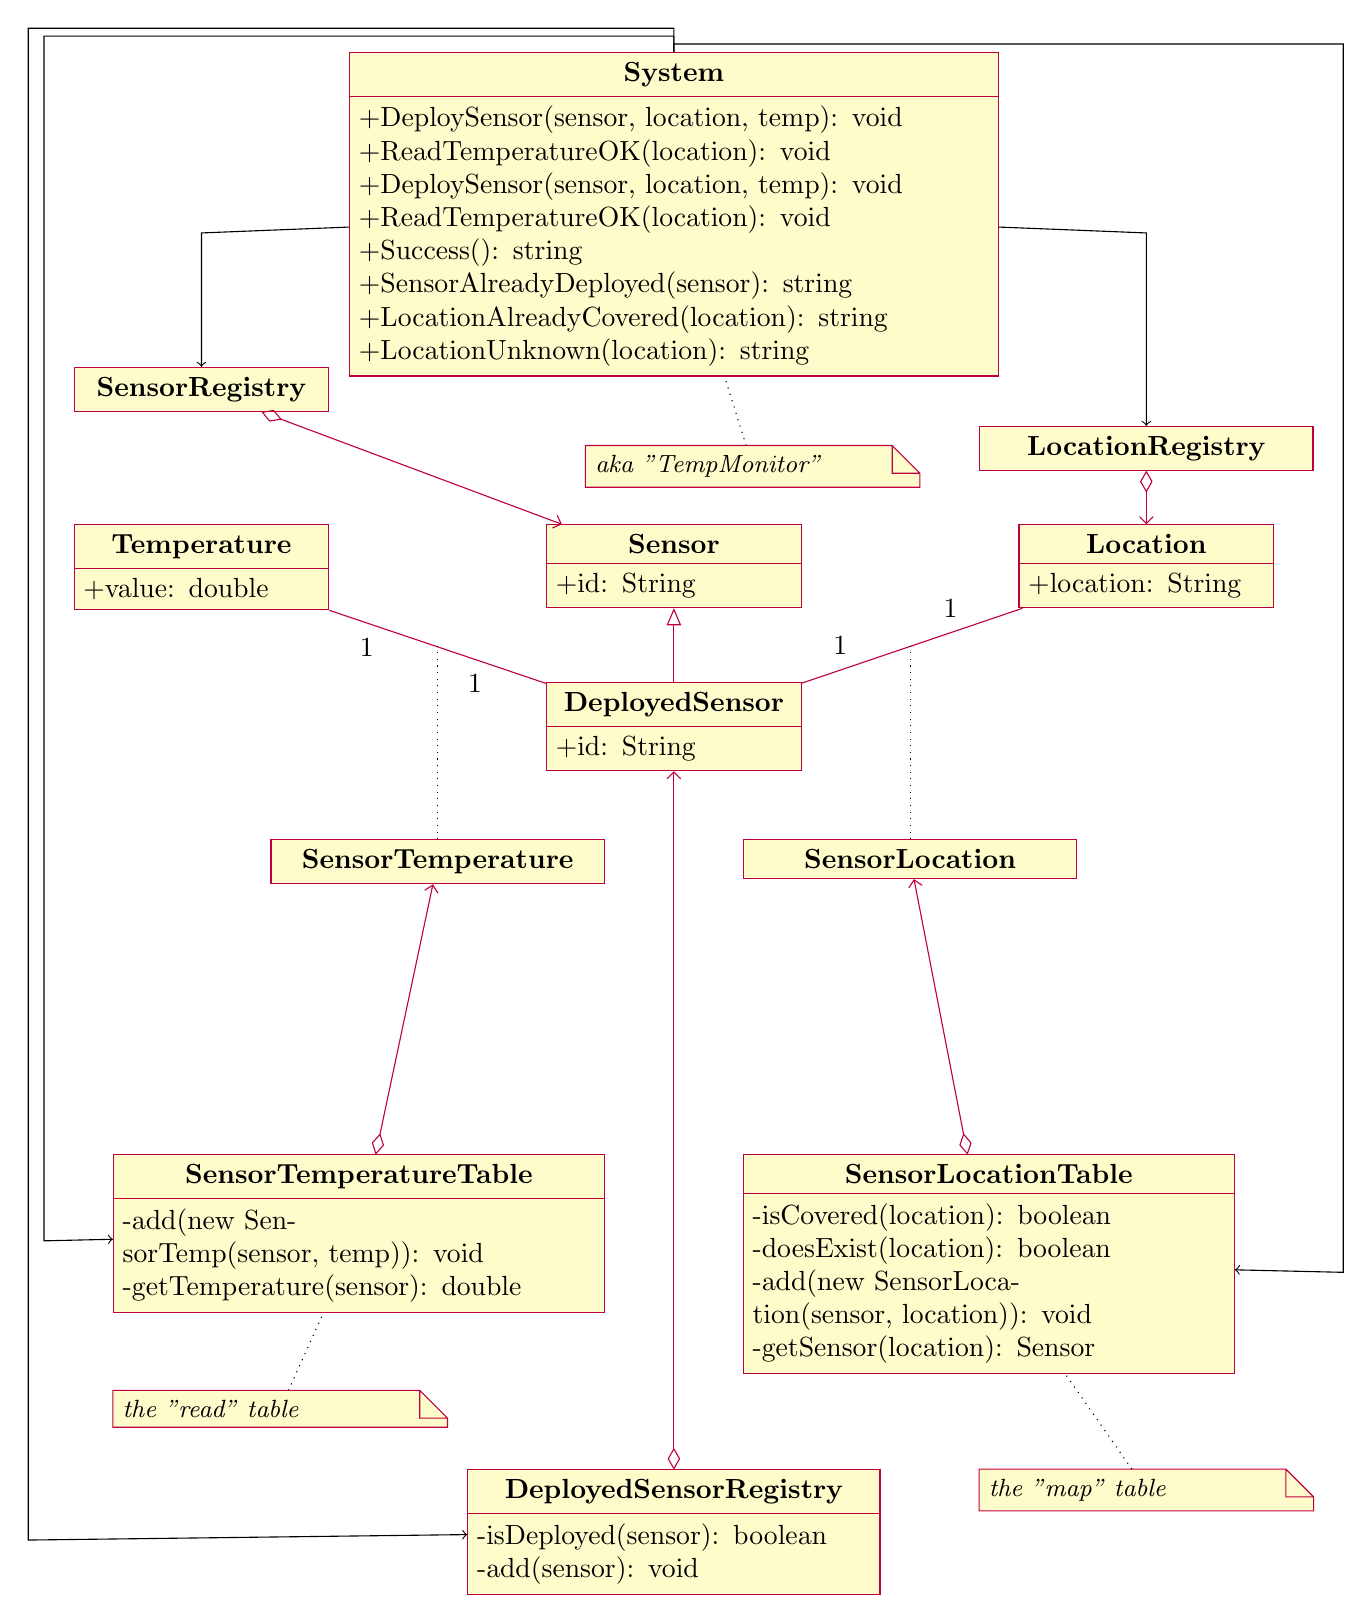
\begin{tikzpicture}

        % Defining the classes and their attributes
        \begin{class}[text width=8cm]{System}{0,6}
            \operation{+DeploySensor(sensor, location, temp): void}
            \operation{+ReadTemperatureOK(location): void}
            \operation{+DeploySensor(sensor, location, temp): void}
            \operation{+ReadTemperatureOK(location): void}
            \operation{+Success(): string}
            \operation{+SensorAlreadyDeployed(sensor): string}
            \operation{+LocationAlreadyCovered(location): string}
            \operation{+LocationUnknown(location): string}
        \end{class}
        
        \begin{class}[text width=3cm]{SensorRegistry}{-6,2}
        \end{class}
        
        \begin{class}[text width=3cm]{Sensor}{0,0}
            \attribute{+id: String}
        \end{class}
        
        \begin{class}[text width=4cm]{LocationRegistry}{6,1.25}
        \end{class}

        \begin{class}[text width=3cm]{Location}{6,0}
            \attribute{+location: String}
        \end{class}
        
        \begin{class}[text width=3cm]{DeployedSensor}{0,-2}
            \inherit{Sensor}
            \attribute{+id: String}
        \end{class}

        \begin{class}[text width=3cm]{Temperature}{-6,0}
            \attribute{+value: double}
        \end{class}

        \begin{class}[text width=4cm]{SensorTemperature}{-3,-4}
        \end{class}

        \begin{class}[text width=4cm]{SensorLocation}{3,-4}
        \end{class}

        \begin{class}[text width=6cm]{SensorTemperatureTable}{-4,-8}
            \operation{-add(new SensorTemp(sensor, temp)): void}
            \operation{-getTemperature(sensor): double}
        \end{class}

        \begin{class}[text width=6cm]{SensorLocationTable}{4,-8}
            \operation{-isCovered(location): boolean}
            \operation{-doesExist(location): boolean}
            \operation{-add(new SensorLocation(sensor, location)): void}
            \operation{-getSensor(location): Sensor}
        \end{class}

        \begin{class}[text width=5cm]{DeployedSensorRegistry}{0,-12}
            \operation{-isDeployed(sensor): boolean}
            \operation{-add(sensor): void}
        \end{class}

        % Defining the links between the classes
        \association {DeployedSensor}{1}{}{Location}{1}{}
        \association {DeployedSensor}{1}{}{Temperature}{1}{}
        \aggregation{SensorRegistry}{}{}{Sensor}
        \aggregation{DeployedSensorRegistry}{}{}{DeployedSensor}
        \aggregation{LocationRegistry}{}{}{Location}
        \aggregation{SensorLocationTable}{}{}{SensorLocation}
        \aggregation{SensorTemperatureTable}{}{}{SensorTemperature}

        % Manual associations
        \draw[->] (System) -- (-6, 3.7) -- (SensorRegistry);
        \draw[->] (System) -- (6, 3.7) -- (LocationRegistry);
        \draw[->] (System) -- (0, 6.1) -- (8.5, 6.1) -- (8.5, -9.5) -- (SensorLocationTable);
        \draw[->] (System) -- (0, 6.2) -- (-8, 6.2) -- (-8, -9.1) -- (SensorTemperatureTable);
        \draw[->] (System) -- (0, 6.3) -- (-8.2, 6.3) -- (-8.2, -12.9) -- (DeployedSensorRegistry);
        \draw[dotted] (SensorTemperature) -- (-3, -1.5);
        \draw[dotted] (SensorLocation) -- (3, -1.5);

        % Notes
        \umlnote(note1) at (1,1){\textit{\small aka "TempMonitor"}};
        \draw[dotted] (note1) -- (System);
        \umlnote(note2) at (-5,-11){\textit{\small the "read" table}};
        \draw[dotted] (note2) -- (SensorTemperatureTable);
        \umlnote(note3) at (6,-12){\textit{\small the "map" table}};
        \draw[dotted] (note3) -- (SensorLocationTable);
    
    \end{tikzpicture}
\end{document}
